\section{Segmentation}

Segmentation is the process of dividing an image into distinct regions that should represent the objects in the image. For example in an application that monitors traffic congestion on a road, it would be useful count the number of cars in a video frame. To do this it’s important to distinguish between groups of pixels that belong to the background and those that belong to cars.

This application concerns itself with distinguishing between pixels that belong to healthy skin surrounding a lesion, and those that belong to the lesion itself.

\subsection{Thresholding}

Thresholding describes a family of segmentation techniques that group neighbouring pixels together based on the similarity of their intensity. Basically the image is converted to a greyscale image and pixels grouped based on whether their are above or below a ratio, and if they are adjoining.

The following figures \ref{fig:thresh_A} to \ref{fig:thresh_D} are examples of segmentation using thresholding with threshold values at 39\% and 50\%. The regions are grouped together based on adjacency and colour coded. Before thresholding, the images were equalised using CLAHE.

\begin{figure}[H]
    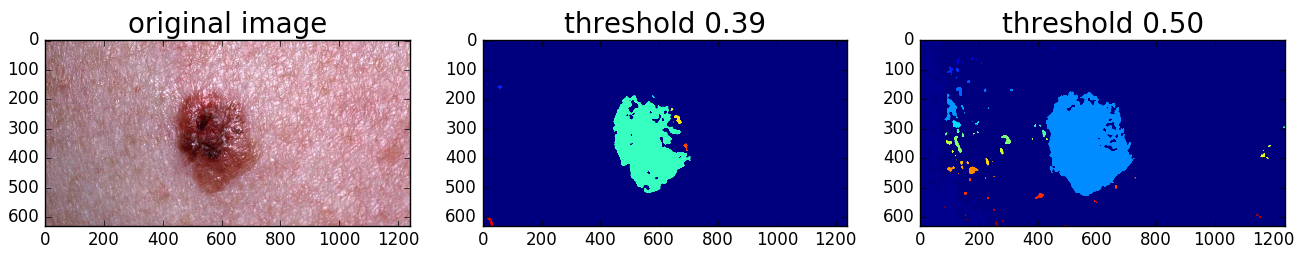
\includegraphics[width=\textwidth,keepaspectratio]{assets/image_processing/thresholding/figure_01.png}
    \caption{Threshold segmentation A}
    \label{fig:thresh_A}
\end{figure}
\begin{figure}[H]
    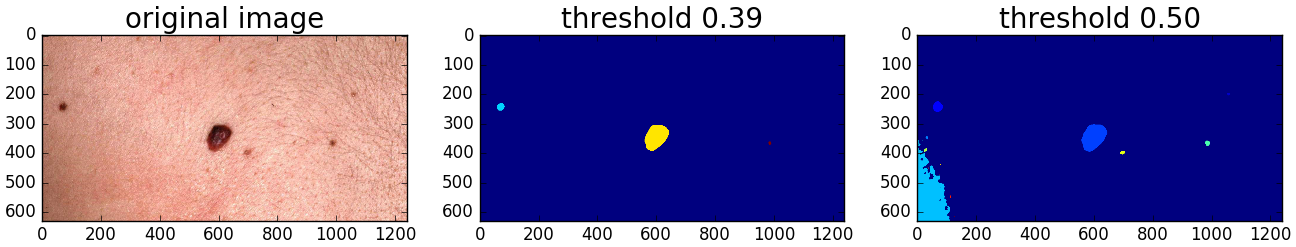
\includegraphics[width=\textwidth,keepaspectratio]{assets/image_processing/thresholding/figure_02.png}
    \caption{Threshold segmentation B}
    \label{fig:thresh_B}
\end{figure}
\begin{figure}[H]
    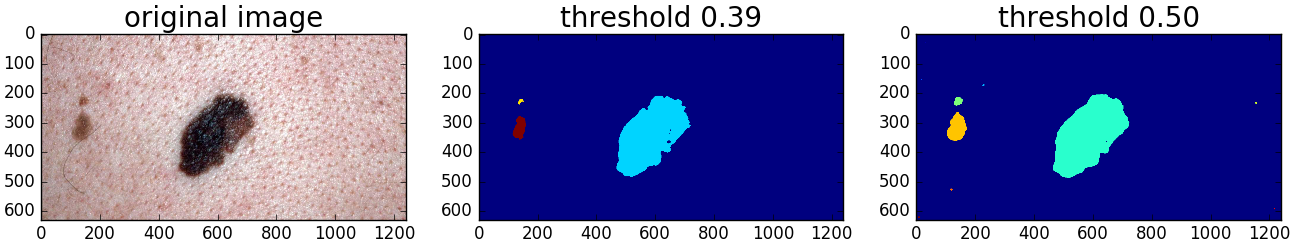
\includegraphics[width=\textwidth,keepaspectratio]{assets/image_processing/thresholding/figure_03.png}
    \caption{Threshold segmentation C}
    \label{fig:thresh_C}
\end{figure}
\begin{figure}[H]
    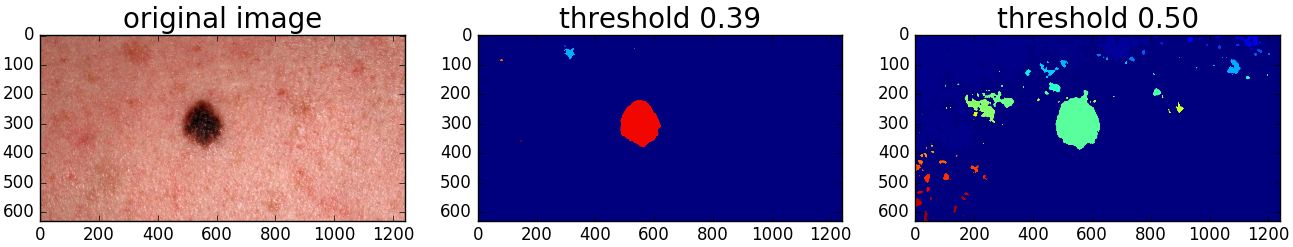
\includegraphics[width=\textwidth,keepaspectratio]{assets/image_processing/thresholding/figure_04.png}
    \caption{Threshold segmentation D}
    \label{fig:thresh_D}
\end{figure}

Depending on the content of the image and the threshold value used more regions are isolated than actually needed. It is fairly easy to discard the irrelevant regions based on some simple assumptions. We can assume that the most interesting region should be roughly in the center of the image, it should be larger than other regions, and it should not touch the edge of the image. The region remaining should be the main region of interest.

Other problems remain though. The regions of interest in figures \ref{fig:thresh_A} and \ref{fig:thresh_C} have some holes within the main region. Figure \ref{fig:thresh_D} has too much area selected at the higher threshold value, \ref{fig:thresh_A} has too little at the lower threshold setting. A static threshold setting will generally not achieve the same level of quality for all images.

By measuring the size of the main region of interest at different threshold values.

\subsection{Color Transformation and Analysis}

\begin{figure}[H]
    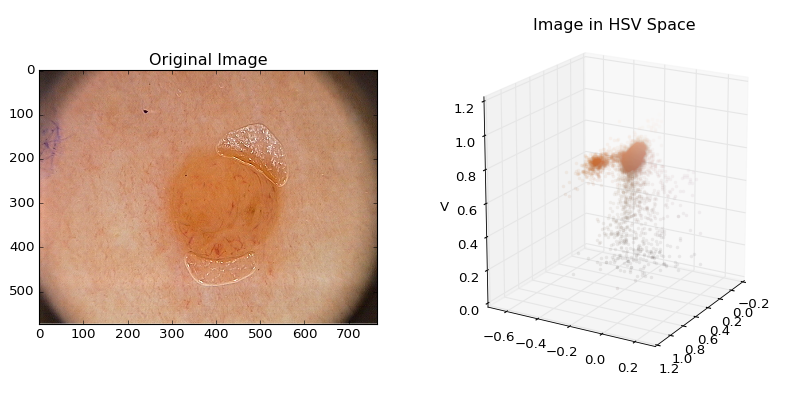
\includegraphics[width=\textwidth,keepaspectratio]{assets/image_processing/hsv/hsv_3dplot.png}
    \caption{HSV Space}
    \label{fig:hsv_place}
\end{figure}

\begin{figure}[H]
    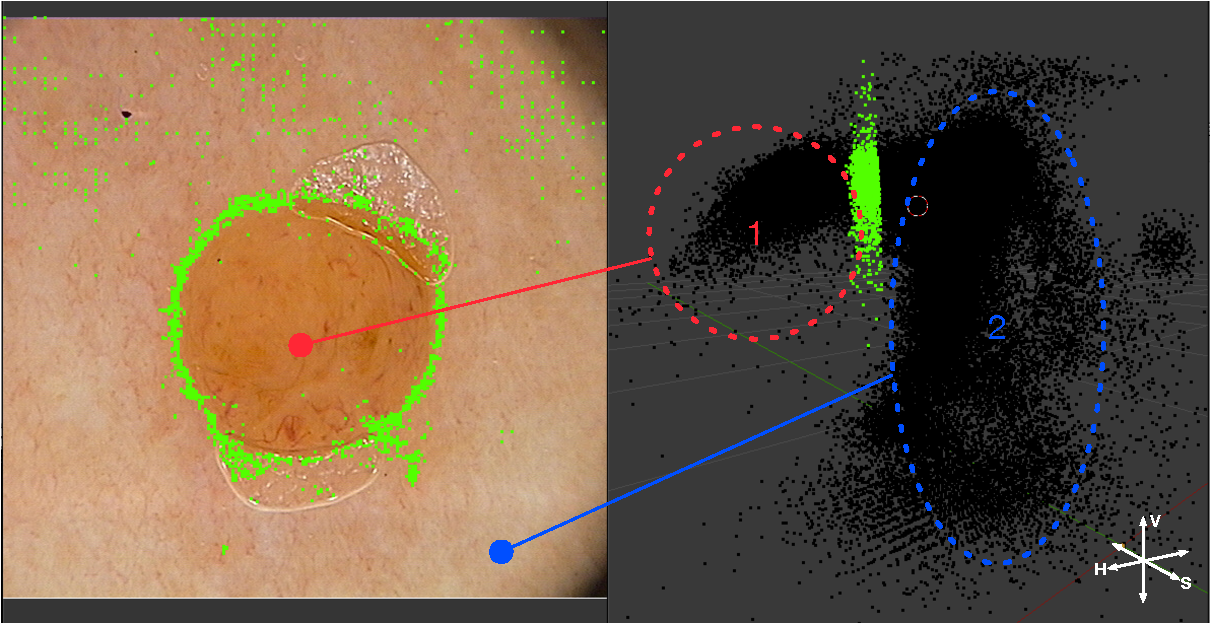
\includegraphics[width=\textwidth,keepaspectratio]{assets/image_processing/hsv/hsv_space.pdf}
    \caption{HSV Clustering visualization}
    \label{fig:hsv_3d}
\end{figure}



\subsection{Super Pixels}
